\chapter{Layout Languages as Sugared Attribute Grammars}
\section{Motivation and Approach}

We start by examining challenges for building layout languages and our high-level solution of automation through attribute grammars.  Throughout this and the remaining chapters, we focus on the design and implementation of one simple layout widget. We will show how our support of it generalizes to common layout languages and, more generally, computations over trees.

\subsection{Important properties for layout languages and others}
Layout languages are some of the most common -- for one gauge, there are over 634 million websites live in 2012, with 51 million added that year~\footnote{http://news.netcraft.com/archives/2012/12/04/december-2012-web-server-survey.html}. Beyond the CSS and HTML languages used for webpage layout, designers also use \LaTeX~[[CITE]] for document layout, D3~[[CITE]] for data visualization, Swing~[[Swing]] for GUI layout, and even specialize within these domains such as by using markdown for text. 


Popular layout languages foster designer productivity by providing abstractions that are rich and numerous.
The alternative is analogous to asking a programmer to write in a low-level language such as assembly: designers should not manually specify, for each element, the position on a canvas and the style. Instead, layout languages resemble constraint systems where designers  declare high-level properties. For example, the high-level program \code{hello world} states that the words \code{hello} and \code{world} should be rendered, and word \code{world} should follow line-wrapping rules for its positioning after \code{hello}. Layout languages may provide quite complicated constraints -- for example, most document layout languages resort to defining their line wrapping rule  in a flexible low-level language. Likewise, they may provide many featuress, such as in the 250+ pages of rules for the CSS language. Adding to the sophistication, many languages support designers adding their own constraints, such as through macros in \LaTeX,  percentage constraints in CSS, and arbitrary functions in Adobe Flex~[[CITE]]. 

The richness of popular layout languages comes at the cost of of complicating their design and implementation:

\begin{itemize}
\item \textbf{Safe semantics.} Does every input layout have exactly one unique rendering? Are the constraints restricted enough such that an efficient implementation is feasible for low-power devices, big data sets, and fast animation? When a feature is added, does it conflict with anything of the above properties? We want an automated way to verify such properties.
\item \textbf{Safe implementation.} As a layout language grows in popularity, it grows in features. Likewise, developers will port it to many platforms and optimize it, and in cases such as CSS, reimplement it from scratch. Does the implementation conform to the intended semantics? Conformance bugs for CSS plague developers~[[CITE]], and failures to match {\LaTeX}'s semantics have killed multiple attempts to modernize the implementation. We want an automated way to ensure that the implementation matches the specification.
\item \textbf{Advanced implementation.} Layout languages tend to add feature as they evolve. However, the implementation of each feature also has demands that increase with time: improved speed and memory footprint, better debugging support, etc. Browser layout engines for CSS are currently over 100,000 lines of optimized C++ code, and most rich layout languages thus far have resisted parallelization. We want automation techniques to lower the implementation burden and more aggressively target those goals.
\end{itemize}


\begin{figure}
\centering
\includegraphics[trim=0 0 0 0,clip,width=1.0\columnwidth]{chapter2/architecture}
\caption{\textbf{Layout engine architecture.} }
\label{fig:architecture}
\end{figure}

Our idea is to declaratively specify layout languages and automatically compile them into an efficient implementation. At runtime, an instance of layout will be processed through the previously generated layout engine (Figure~\ref{fig:architecture}). The compiler is responsible for checking the semantics of the layout features and, by construction, provides a correct implementation. Furthermore, instead of manually optimizing the code for every individual feature, language designers instead write generic compiler optimizations. As a similar implementation benefit, we automatically target multiple platforms for the same layout language, such as scripting languages in order to use their debuggers, and multicore and GPU languages to gain magnitudes of speedups.

We show that the attribute grammar formalism supports specification of layout languages. It is unclear how to encode complicated layout language features with the traditional formalism, so we support a rich form of attribute grammars and reduce reasoning about them to handling a more traditional formalism (reducer in Figure~\ref{fig:architecture}). The remainder of this chapter introduces the high-level attribute grammar formalism, how to specify layout languages using it, and an intuition for the reduction into a lower-level formalism.


\newsavebox{\agdef}
\begin{lrbox}{\agdef}% Store first listing
\begin{minipage}{1\columnwidth}
\setlength{\grammarparsep}{0.15cm}   % vertical distance between production rules
\setlength{\grammarindent}{1cm}
\renewcommand{\litleft}{\bfseries}
\renewcommand{\ulitleft}{\bfseries}
\renewcommand{\superscript}[1]{\ensuremath{^{\textrm{#1}}}}
\renewcommand{\subscript}[1]{\ensuremath{_{\textrm{\uppercase{#1}}}}}
\renewcommand{\syntleft}{\normalfont\itshape}
\renewcommand{\syntright}{}
%\newcommand{\deriv}{~::=~}
\renewcommand{\deriv}{~ $\rightarrow$ ~}
\begin{grammar}
<AG> \deriv{} (<Prod> "\{" <Stmnt>? "\}")*

<Prod> \deriv{} <V> $\rightarrow$ <V>*

<Stmnt> \deriv{} <Attrib> "=" <id>(<Attrib>*) ~  | ~ <Attrib> "=" <n> ~ | ~ <Stmnt> ; <Stmnt> 

<Attrib> \deriv{} <id>.<id>
\end{grammar}
\end{minipage}
\end{lrbox}



\newsavebox{\hboxtreetext}
\begin{lrbox}{\hboxtreetext}% Store first listing
\begin{lstlisting}[language=C++,morekeywords={spawn,join,reverse,parallel_for}]
<S>
  <HBox name=child>
    <HBox name=left>
      <HBox name=left w=20 h=5/>
      <HBox name=right w=15 h=5/>
    </HBox>
    <HBox name=right w=15 h=5/>
  </HBox>
</S>
\end{lstlisting}
\end{lrbox}


\begin{figure}
\subfloat[\textbf{Input tree.} Only some of the x, y, w, and h attributes are specified.]{\label{fig:hbox:input}
\begin{minipage}{1\columnwidth}\centering
\includegraphics[trim=0 0 0 0,clip,width=0.6\columnwidth]{chapter2/output}
\end{minipage}}\\
\subfloat[\textbf{Textual encoding of input tree.}]{\label{fig:hbox:texttree}
\begin{minipage}{1\columnwidth}\centering
\usebox{\hboxtreetext}
\end{minipage}
}\\
\subfloat[\textbf{Attribute grammar for a language of horizontal boxes.}]{\label{fig:hbox:grammar}
\begin{minipage}{1\columnwidth}
\begin{grammar}
<S> \deriv{} \emph{HBOX} \\ 
  \{ HBOX.x = 0; HBOX.y = 0 \}

<HBOX> $\rightarrow$ $\epsilon$  \\
\{ HBOX.w = input$_w$(); HBOX.h = input$_h$() \} 

<HBOX$_0$> $\rightarrow$ \emph{HBOX$_1$} \emph{HBOX$_2$} \\
\{ HBOX$_1$.x = HBOX$_0$.x; \\
$~~~$ HBOX$_2$.x = HBOX$_0$.x + HBOX$_1$.w; \\
$~~~$ HBOX$_1$.y = HBOX$_0$.y; \\
$~~~$ HBOX$_2$.y = HBOX$_0$.y; \\
$~~~$ HBOX$_0$.h = max(HBOX$_1$.h, HBOX$_2$.h); \\
$~~~$ HBOX$_0$.w = HBOX$_1$.w + HBOX$_2$.w \} 
\end{grammar}
\end{minipage}
}\\
\subfloat[\textbf{Language of attribute grammars.}]{\label{fig:ag}
\usebox{\agdef}
}
\caption{For a language of horizontal boxes: (a) input tree to solve and (b) attribute grammar specifying the layout language. Specification language of attribute grammars shown in (c).%and (c) dynamic data dependencies.
}
\label{fig:hbox}
\end{figure}


\section{Background: Layout with Classical Attribute Grammar}

This section describes specifying a simple layout language as an attribute grammar and two classical implementation strategies. We reuse the example throughout our work to explore various concepts.



\subsection{Attribute Grammars}

Consider solving the tree of horizontal boxes shown in Figure~\frefb{fig:hbox}{fig:hbox:input}. As input, a webpage author provides a tree with constraints (Figure~\frefb{fig:hbox}{fig:hbox:text tree}). Only some node attribute values are provided: in this case, only the widths and heights of leaf nodes. The meaning of a horizontal layout is that, as is visualized, the boxes will be placed side-by-side. The layout engine must solve for all remaining x, y, width, and height attributes. 

We declaratively specify the layout language of horizontal boxes, \hlang{},  as shown in Figure~\frefb{fig:hbox}{fig:hbox:grammar}, with an attribute grammar~\cite{oag,Meyerovich:2010,htmlag}. First, the specification defines the set of well-formed input trees as the derivations of a context-free grammar. We use the standard notation~[[CITE]]. In this case, a document is an unbalanced binary tree of arbitrary depth where the root node has label \texttt{S} and intermediate nodes have label \texttt{HBOX}. Second, the specification defines semantic functions that relate attributes associated with each node. For example, the width of an intermediate horizontal node is the sum of its children widths. Likewise, the width of a leaf node is provided by the user, which is encoded by the nullary function call $input_w()$:


\begin{grammar}
<HBOX> $\rightarrow$ $\epsilon$ \{ HBOX.w = $input_w$(); $\ldots$ \} ~~~~~~~~~~~~~~~~~~~~~~~ /* leaf */

<HBOX$_0$> $\rightarrow$ \emph{HBOX$_1$} \emph{HBOX$_2$} ~~~~~~~~~~~~~~~~~~~~~~~~~~~~~~~~~ /* binary node */\\
\{ $\ldots$ HBOX$_0$.w = HBOX$_1$.w + HBOX$_2$.w \} 
\end{grammar}


The specification intentionally does not define the evaluation order. For example, the specification does not state whether to compute a node's width before its height. Likewise, our optimized approach will compute the attributes as a sequence of tree traversals, but the specification does not state what those traversals are. Leaving the evaluation order unspecified provides freedom for our compilers to pick an efficient parallel order. Irrespective of whatever evaluation order is ultimately used to solve for the attribute values, the statements define constraints that must hold over the computed result. Attribute grammars can therefore be thought of as a single assignment language where attributes are dataflow variables~[[CITE]].


The language of attribute grammars is defined in Figure~\frefb{fig:hbox}{fig:ag}. In addition the defining the context free grammar, it supports single-assignment constraints over attributes of nodes in a production. Our example uses the following encoding. Semantic functions are pure and left uninterpreted, so, for example, we encode the addition of widths as ``\mbox{HBOX$_0$.w = f(HBOX$_1$.w, HBOX$_2$.w)}''. Our program analysis techniques do not need to know the contents of the function, just that the output of a call depends purely on the inputs.  For the same reason, we encode constant values as nullary function calls. 

To specify grammars more complicated than \hlang{}, we describe linguistic extensions for richer functional specifications (Section~\ref{sec:desugaring}) and, to control the evaluation order, behavioral specification (Chapters~\ref{chap:3} and \ref{chap:4}).

\begin{figure}
\subfloat[Initial dependencies.]{\label{fig:deps:full}
\begin{minipage}{0.5\columnwidth}\centering
\includegraphics[trim=0 0 0 0,clip,width=1.0\columnwidth]{chapter2/deps}
\end{minipage}}
\subfloat[After first round of evaluation.]{\label{fig:deps:step}
\begin{minipage}{0.5\columnwidth}\centering
\includegraphics[trim=0 0 0 0,clip,width=1.0\columnwidth]{chapter2/depsstep}
\end{minipage}}
\caption{\textbf{Dynamic data dependencies and evaluation}. Shown for constraint tree  in Figure~ZZZ~(a). Circles denote attributes, with black circles denote attributes with resolved dependencies such as \sched{input()}s. Thin lines show data dependencies and thick lines show production derivations. Second chart shows the dependency graph resulting from evaluating all source nodes and marking them as resolved.}
\label{fig:deps}
\end{figure}


\subsection{Dynamic data dependencies and dynamic evaluation}
A simple and classic evaluation strategy is to \emph{dynamically} compute over a tree. The evaluator dynamically follows the dynamic data dependencies between instances of attributes. The dynamic evaluation strategy is too slow for our use cases, but it introduces the key concepts of dynamic data dependencies, the dynamic semantics of attributes grammars, and the corresponding dynamic interpreter.

An instance of a document corresponds to the dependency graph shown in Figure~\frefb{fig:reps}{fig:deps:full}. Each attribute of a tree node is either a source, meaning its value can be computed based on other known values, or it cannot be evaluated until other attribute values are known. It is a dynamic dependency graph in that each data dependency in the static code may be instantiated as multiple data dependencies given a tree at runtime. 

The dynamic data dependency graph leads to a simple semantics for the result of evaluation. The graph corresponds to a system of equations where edges link instance variables. For example, static code \code{HBOX$_2$.x = HBOX$_0$.x + HBOX$_1$.w} instantiates twice for the Figure~\frefb{fig:deps}{fig:reps:full}: once for each $x$ attribute with an incoming elbow connector. The value of both $x$s are constrained by distinct instances of the above constraint. If the dependency graph is a directed acyclic graph and each attribute appears on the lefthand side of exactly one equality statement (\emph{dataflow variables}), there is exactly one solution to the system of equations.

A simple procedure solves an instance of a system of equations: topological traversal. The algorithm is as follows:
\begin{figure}
\begin{lstlisting}[mathescape,language=C++,morekeywords={for,in,where,input,output,repeat,until,return}]
input: $G = (V,E)$
output: $Map$
$Map \leftarrow \emptyset$
$E' \leftarrow E$
$V' \leftarrow V$
for $a \in V' \texttt{where} \not\exists (n,a) \in E'$:
  $Map \leftarrow Map \cup \{a \rightarrow \texttt{eval}(a)\}$
  $V' \leftarrow V' - a$
  $E' \leftarrow E' \ (\{a\} \times V)$
repeat until $E' = \emptyset$
return $Map$
\end{lstlisting}
\caption{\textbf{Dynamic attribute grammar evaluator.} It selects attributes in a safe order by dynamically removing dependency edges as they are resolved. }
\label{fig:dyneval}
\end{figure}
The algorithm literately finds an attribute whose dependencies have all been previously resolved, evaluates the attribute, and repeats. If the input graph is a directed acyclic graph, this procedure is guaranteed to terminate. The insight is that a directed acyclic graph has at least one fringe node, the loop removes them, and removing these nodes yields a smaller directed acylic graph.

The dynamic evaluation strategy provides a small explanation for the natural semantics, but it leaves several challenges. First, runtime manipulation of a dynamic dependency graph introduces high overheads because every dynamic dependency edge must be manipulated. Second, it is unsafe. For example, a cycle in the dependency graph causes the above evaluation strategy to get stuck, so dynamic evaluators must introduce runtime cycle check. Designers can build layout widgets that, depending on how they are invoked, fail to display!

%\subsection{Static data dependencies and static evaluators}




\section{Desugaring Loops and Other Modern Constructs}
\label{sec:desugaring}

The attribute grammar formalism was invented for describing semantics~[[CITE]] and before many modern constructs became mainstream: we had to design extensions for improved expressiveness and maintainability. Our extensions exploit concepts from structured, object-oriented, and functional programming. Other language designers have build such extensions as well~[[CITE]]: our challenge was to make expressive extensions that facilitate effective parallelization and do not overly complicate language and tool implementation. This section documents the language features and how they simplify implementation, and leaves performance optimization to the next chapter.

Our key insight is that pre- and post-processing supports desugaring a feature-rich attribute grammar into the canonical attribute grammar notation. Tools then operate at the most appropriate stage, such as our scheduler on the small, canonical attribute grammar representation. Likewise, our code generators take a generated schedule and relate it back to a representation from early in the preprocessing stage. Many of the below features are built as explicit compiler stages, but over time, we found that declarative tree rewriting systems such as ANTLR and OMeta support automating individual stages.



\newsavebox{\ifacegrammar}
\begin{lrbox}{\ifacegrammar}% Store first listing
\begin{lstlisting}[language=C++,morekeywords={interface,class,children}]
interface BoxI { }
class HBoxLeaf : BoxI { }
class HBoxBinary : BoxI { 
  children {
    left: BoxI;
    right: BoxI;
  }
}
class VBoxLeaf : BoxI { }
class VBoxBinary : BoxI { 
  children {
    left: Box;
    right: Box;
  }
}
\end{lstlisting}
\end{lrbox}




\begin{figure}
\subfloat[\textbf{Canonical attribute grammar.}]{\label{fig:iface:problem}
\begin{minipage}{1\columnwidth}
\begin{grammar}
<S> \deriv{} \emph{HBOX}  $|$  \emph{VBOX}

<HBOX> \deriv{} $\epsilon$  

<HBOX$_0$> \deriv{} \emph{HBOX$_1$} \emph{HBOX$_2$} 

<HBOX$_0$> \deriv{} \emph{VBOX$_1$} \emph{HBOX$_2$} 

<HBOX$_0$> \deriv{} \emph{HBOX$_1$} \emph{VBOX$_2$} 

<HBOX$_0$> \deriv{} \emph{VBOX$_1$} \emph{VBOX$_2$} 

<VBOX> \deriv{} $\epsilon$  

<VBOX$_0$> \deriv{} \emph{HBOX$_1$} \emph{HBOX$_2$} 

<VBOX$_0$> \deriv{} \emph{VBOX$_1$} \emph{HBOX$_2$} 

<VBOX$_0$> \deriv{} \emph{HBOX$_1$} \emph{VBOX$_2$} 

<VBOX$_0$> \deriv{} \emph{VBOX$_1$} \emph{VBOX$_2$} 

\end{grammar}
\end{minipage}
}\\
\subfloat[\textbf{Interface sugar.}]{\label{fig:iface:clean}
\usebox{\ifacegrammar}
}\\
\subfloat[\textbf{Interface encoding.}]{\label{fig:iface:rewrite}
\begin{minipage}{1\columnwidth}
\begin{grammar}
<S> \deriv{} \emph{BOX}

<BOX> \deriv{} \emph{HBOX} $|$ \emph{VBOX}

<HBOX> \deriv{} $\epsilon$  

<HBOX$_0$> \deriv{} \emph{BOX$_1$} \emph{BOX$_2$} 

<VBOX> \deriv{} $\epsilon$  

<VBOX$_0$> \deriv{} \emph{BOX$_1$} \emph{BOX$_2$} 

\end{grammar}
\end{minipage}
}
\caption{\textbf{Interfaces for tree grammars}. Subfigures show manually encoding multiple production right-hand sides, an encoding that uses a \code{Box} non-terminal for indirection, and the high-level encoding using interfaces and classes.}
\label{fig:iface}
\end{figure}


\begin{figure}
\begin{lstlisting}[language=C++,morekeywords={spawn,join,reverse,parallel_for}]
{"class": "HBox",
 "children": {
   "left": {
     "class": "HBox",
     "children": {
       "left":  {"class": "HBox", "w": 20, "h": 5},
       "right": {"class": "HBox", "w": 15, "h": 5}}},
   "right": {
     {"class": "HBox", "w": 15, "h": 5}}}}
\end{lstlisting}
\caption{\textbf{Input tree as graph with labeled nodes and edges}. Specified in the JSON notation.}
\label{fig:hboxjson}
\end{figure}

\subsection{Interfaces for Encoding Tree Grammars}
Attribute grammars are an extension to the tree grammar formalism for defining input trees, so improving the abstraction capabilities of tree grammars also aids the ability to structure attribute grammars. In particular, we found the need to support  abstracting over similar types of non-terminals. Our solution is to provide a notion of classes and interfaces. Our core extension is macro-expressible with attribute grammars and therefore reduces implementation requirements, though it is still important enough that it merits deeper compiler support. 


Consider the code duplication performed when extending \hlang with vertical boxes. The children of a \code{HBox} could be a horizontal box or a vertical box, and the same for the children of a vertical box. Figure~\ref{fig:face:problem} shows that the 3 productions of \hlang grew to be 11. The example highlights that canonical attribute grammars cannot abstract over node types. Adding a new box type requires modifying all previous box classes, and in the presence multiple children, extension suffers exponential costs. 

To abstract over node types, we introduce the notion of classes and interfaces (Figure~\ref{fig:iface:clean}). Classes are similar to the productions of an attribute grammar: the class name specifies the production's lefthand side non-terminal and the children block specifies the production's righthand side. Unlike attribute grammars, an interface name is used for the righthand side rather than the class name. \code{HBox} and \code{VBox} implement interface \code{BoxI}, so any class specified to have a \code{BoxI} child can have a \code{HBox} or \code{VBox} child within the concrete tree. 


Classes and interfaces are formally equivalent to tree grammars in the sense of a 1-to-1 correspondence between trees described by both. First, a tree grammar can be expressed with classes and interfaces by treating all productions with the same lefthand-side non-terminal as different classes belonging to the same interface. In the other direction, each interface can be expressed as a production that derives the classes, and the classes expand into productions. Figures~\ref{fig:iface:clean} and \ref{fig:iface:rewrite} demonstrate the correspondence for \hlang. The induced implementation requirements are therefore slight in the sense that the construct is sugar for a pattern in the canonical attribute grammars. 

We depart from the correspondence for the encoding of trees in two ways. First, we represent input as a tree with labeled nodes and edges. Node labels denote the class and edge labels specify child bindings. Figure~\ref{fig:hboxjson} uses the JSON format common to dynamic languages for an instance of a tree in \hlang. By naming children, such as \code{left} and \code{right}, we eliminate sensitivity to their order within a code block. With order sensitivity, adding a middle child \code{center} would needlessly require refactoring references to the repositioned element \code{right}. Likewise, reordering children in the input data does not require refactoring the attribute grammar.

Our second departure from the canonical attribute grammar encoding optimizes the data representation by eliding intermediate interface nodes. The reduction to attribute grammars suggests adding a new non-terminal for each interface, but doing so in the data representation doubles the number of nodes in the concrete tree. Making the interface pattern a language construct with compiler support eliminates associated costs, such as cutting file size for runtime parsing of big data visualizations.

\begin{figure}
\begin{lstlisting}[language=C++,morekeywords={interface,class,var,input,int,float}]
interface BoxI {
  var x : float;
}
class HBoxLeaf : BoxI {
  attributes {
    var y : int;
    input w : ? int;
    input h : int = 10;
  }
}


\end{lstlisting}
\caption{\textbf{Input tree as graph with labeled nodes and edges}. Specified in the JSON notation.}
\label{fig:hboxjson}
\end{figure}


\subsection{Interfaces for attributes and information hiding.}
Our system provides lightweight specification annotations for different types of attributes, and coupled with the interface construct, it supports defining relationships between attributes across different classes.

Each static attribute is annotated with its assignment type and its embedded value type:
\begin{itemize}
\item \textbf{Assignment types.}
The assignment type denotes whether the input tree defines the value, such as in \code{input w}, or whether the attribute grammar defines it, as in \code{var x}. Assignments to an input type are illegal, and multiple assignments to a variable type are also illegal. 

If an input tree fails to provide an input attribute, a runtime error will be thrown. To still provide an interpretation of such trees, input attributes  support the annotation ''?'',  which enables pattern matching through functions \code{maybeReady :: -> boolean} and \code{maybeValue :: -> 'a}.  Alternatively, for the common scenario of using a fixed default value, a default value can instead be defined as in \code{input h : int = 10}. If the input tree does not provide the value, the default value will be automatically substituted.

Canonical attribute grammars can encode input attributes in two ways. First, semantic functions with no parameters encode the lack of dependencies. Second, for finite domains, the set of tree grammar productions can expand to include attribute nodes. The second encoding more faithfully describes our approach because, like our system, it feeds into an automatic tree parser generator. For each tree node, our generated parser scans for the expected set of input attributes.

\item \textbf{Value types.} 
The system also supports type annotations used for embeddings. Generated code typically compiles as part of a project in a more static language, such as C++, which require a static type discipline. The annotations can be user-defined, such as OpenGL's \emph{vertex buffer object} \code{VBO}, which is not defined within our system.

Our analyzer ignores the value type annotations such as \code{x : float} and \code{y : int} while the low-level code generator passes along the decorations \code{float} and \code{int}.  The embedded design simplifies implementation because value type checking is performed by the host language's compiler. 
\end{itemize}

In practice, we  use attribute definitions in interfaces for information hiding across classes and lightweight specification of relationships between similar classes. An attribute declared inside of a class is \emph{local} to constraints in the class: only the class's constraints can read or write to the attribute. Conversely, declaring a \emph{var} inside of an interface hints that it is meant to be reused by outside classes, such as part of a tree traversal.

\begin{figure}
\begin{lstlisting}[language=C++,morekeywords={trait,class,attributes,actions}]
trait Rectangle {
  attributes { render : int; }
  actions { render := paintRect(x,y,w,h, "black"); }
}
class HBox(Rectangle) : BoxI { ... }
\end{lstlisting}
\caption{\textbf{Trait construct}. Adds shared rendering code to the HBox class.}
\label{fig:trait}
\end{figure}

\subsection{Traits: Reusing Cross-cutting Code}
As with many object systems, we support a trait construct for cross-cutting code that should be shared across classes. It statically expands like a macro, and therefore provides no formal expressive power. For example, Figure~\ref{fig:trait} defines how to render a rectangle given several attributes, and then adds that functionality to class \code{HBox}. If the language was extended with class \code{VBox}, the class definition of \code{VBox} could also use trait \code{Rectangle}.






\begin{figure}
\begin{lstlisting}[language=C++,morekeywords={spawn,join,reverse,parallel_for}]
interface BoxI {
  var w : int;
  var h : int;
  var right : int;
  var bottom : int;
}
class HBox : BoxI {
  children {
    childs : [ BoxI ]
  }
  actions {
      loop childs {
        w := fold 0 .. self$-.w + childs$i.w;
        h := fold 0 .. max(self$-.h, childs$i.h)
        childs.right := fold x .. childs$-.right + childs$i.w;
        childs.bottom := fold y .. childs$-.bottom + childs$i.h;  
      }
  }
}
\end{lstlisting}
\caption{\textbf{Input tree as graph with labeled nodes and edges}. Specified in the JSON notation.}
\label{fig:loops}
\end{figure}

\subsection{Loops}
We extend our language with declarative loops over the attributes of multiple nodes. They are an expressive extension over the uniform recurrence relations of [[CITE]].

The loop construct, \code{loop}, specifies a block of loop body statements. It acts over a sequence of nodes declared with the same interface, such as \code{childs : [ BoxI ]} in Figure~\ref{fig:loops}. The looping order is restricted to forward iteration, though our approach generalizes to other loop orders.

A statement in a loop body will execute for each element of the list. For example, the following statement assigns the attribute \code{w} the sum of the children widths:
\code{w := fold 0 .. self\$-.w + childs\$i.w}
Similar to array index notation, the suffix on righthand-side variable names for loop statements provide a restricted form of relative indexing for loops. In particular:
\begin{itemize}
\item \$i: the ``current'' loop step
\item \$-: the previous loop step
\item \$\$: the last loop step
\end{itemize}
Use of suffix ``\$-'' in a \code{fold} can be thought of as an accumulator in functional programming. 


One loop statement can refer to the accumulator of another, which fold statements in most languages do not support. For example, two loop counters can be intertwined:
\begin{lstlisting}
loop childs {
  childs.counter1 := fold 0 .. childs$-.counter2 + 1;
}
loop childs {
  childs.counter2 := fold 0 .. childs$-.counter1 + 1;
}
\end{lstlisting}
The programmer does not need to order the statements.  For example, our system infers that the imperative code that implements the above declarations is just one imperative loop that fuses them together. The incorrect alternative of implementing the declarations as a different imperative loop for each would lead to unfulfilled data dependencies. The freedom in statement order supports automatic parallelization, but also allowed programmers choice in how to structure the program once machine considerations were removed.

We reduced scheduling loops to scheduling canonical attribute grammars. Our insight is that, for a restricted language of relative indices, we can schedule several unrolled loop steps and generalize the schedule to the rest. Section~\ref{???} discusses this in more detail. 

\subsection{Embedded Domain Specific Language: Functional Rendering}
We designed our system for interaction with other tools and languages. A key ability is to invoke externally-defined functions, such as \code{max()}  of Figure~\ref{fig:loops} for the maximum of two numbers and \code{paintRect()} of Figure~\ref{fig:trait} to draw a rectangle to the screen. Attribute grammars are compiled to run in some host system, such as JavaScript or OpenCL, and any function in scope to the generated code may be called.

Functions can be safely embedded as long as they provide a \emph{pure} interface. In particular, the returned output should only depend on the inputs. Likewise, functions should be reentrant for use in automatic parallelization In the case of embedding in statically checked languages, the host's static checker is responsible for checking usage.



\begin{figure}
\subfloat[\textbf{Sunburst}]{\label{fig:renderings:sunburst}
\begin{minipage}{0.5\columnwidth}\centering
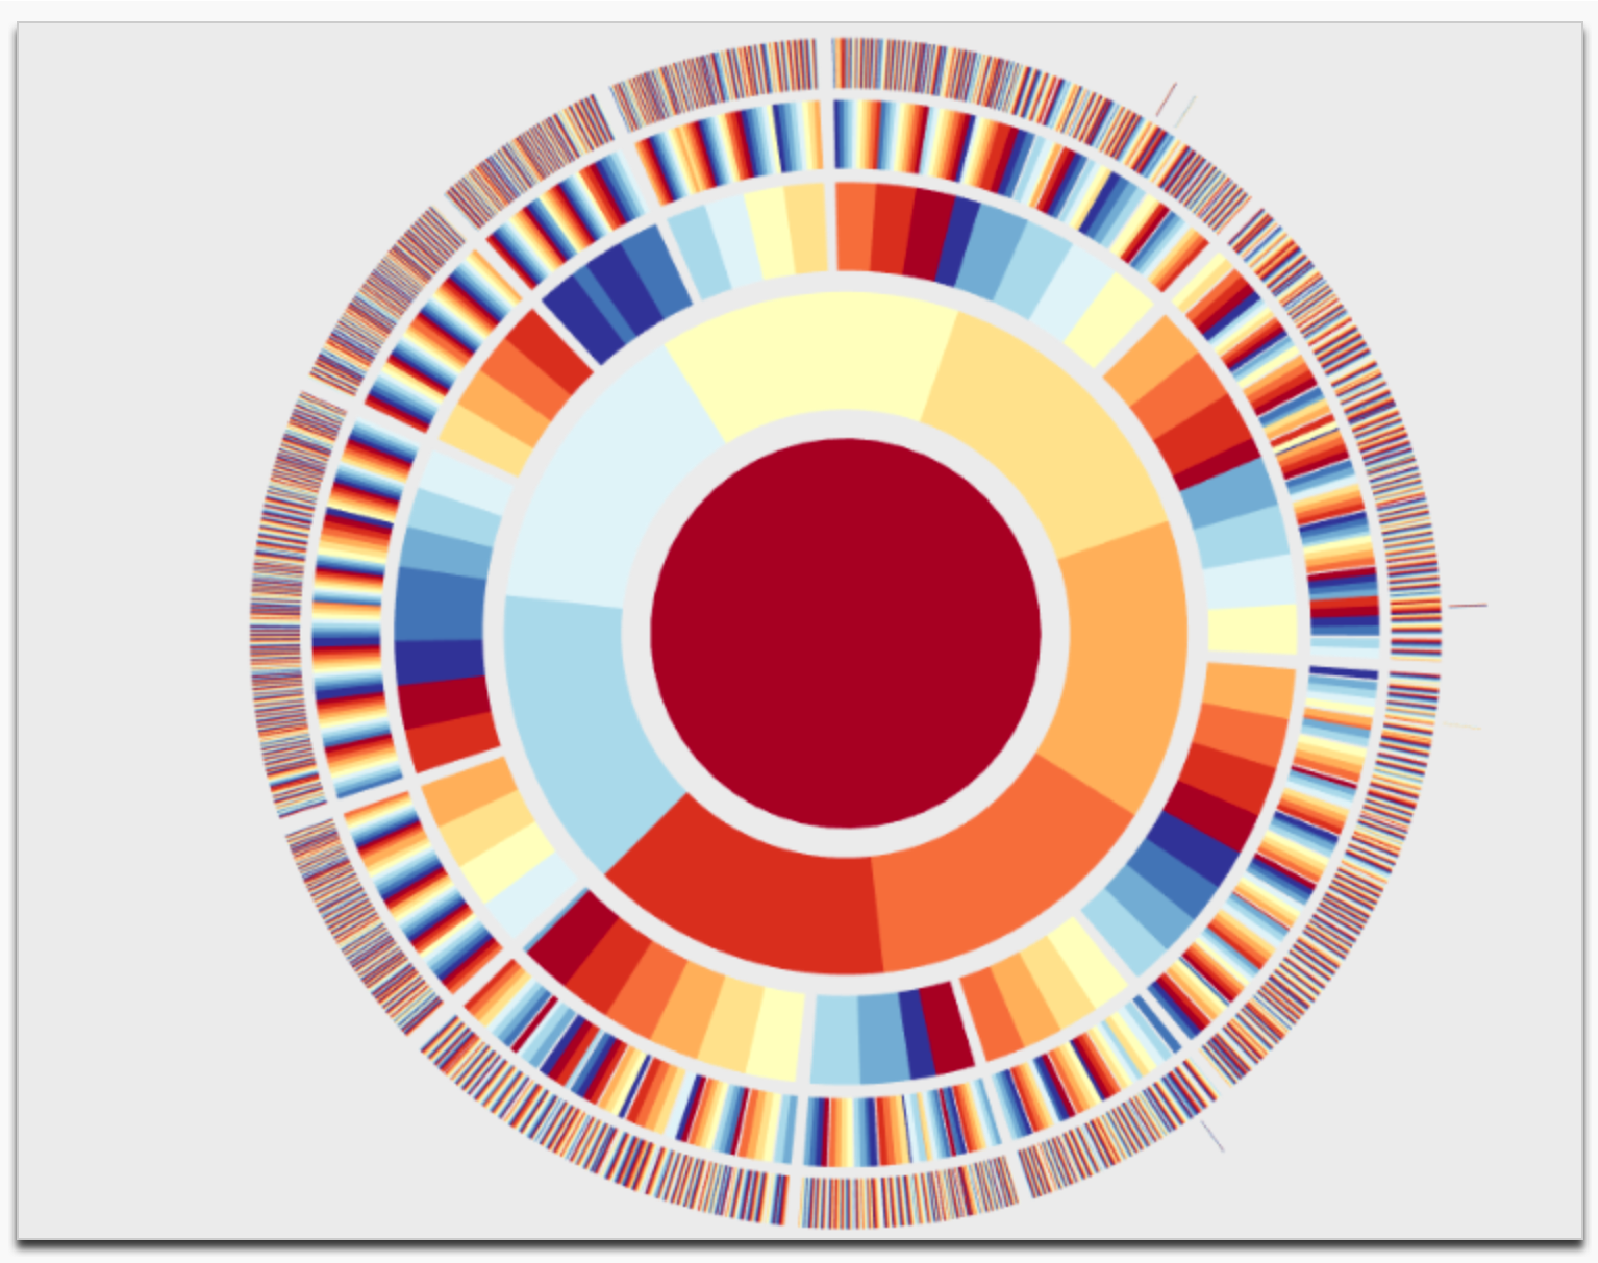
\includegraphics[trim=0 0 0 0,clip,width=1.0\columnwidth]{chapter2/sunburst}
\end{minipage}}
\subfloat[\textbf{Treemap}]{\label{fig:renderings:treemap}
\begin{minipage}{0.5\columnwidth}\centering
\includegraphics[trim=0 0 0 0,clip,width=1.0\columnwidth]{chapter2/election}
\end{minipage}}\\
\subfloat[\textbf{Linked Scatter}]{\label{fig:renderings:parlab}
\begin{minipage}{0.5\columnwidth}\centering
\includegraphics[trim=0 150mm 0 0,clip,width=1.0\columnwidth]{chapter2/parlabscreenshot2}
\end{minipage}}
\subfloat[\textbf{3D Multiple Time Series}]{\label{fig:renderings:ge}
\begin{minipage}{0.5\columnwidth}\centering
\includegraphics[trim=0 0 0 0,clip,width=1.0\columnwidth]{chapter2/ge}
\end{minipage}}\\
\subfloat[\textbf{Line Graph}]{\label{fig:renderings:line}
\begin{minipage}{1.0\columnwidth}\centering
\includegraphics[trim=0 0 0 0,clip,width=0.35\columnwidth]{chapter2/line}
\end{minipage}}
\caption{\textbf{Visualization screenshots.} All except [[CITE]] are interactive or animated. Each one was declaratively specified with our extended form of attribute grammars and automatically parallelized. Labels describe whether GPU or multicore code generation was used.}
\label{fig:vizrenderings}
\end{figure}

\begin{figure}
\subfloat[\textbf{HTML Tables} (grid-based)]{\label{fig:renderings:tables}
\begin{minipage}{1.0\columnwidth}\centering
\includegraphics[trim=0 0 0 0,clip,width=0.3\columnwidth]{chapter2/table}
\end{minipage}}\\
\subfloat[\textbf{CSS} (flow-based)]{\label{fig:renderings:css}
\begin{minipage}{1.0\columnwidth}\centering
\includegraphics[trim=0 0 0 0,clip,width=0.8\columnwidth]{chapter2/wiki}
\end{minipage}}
\caption{\textbf{Document layout screenshots.}}
\label{fig:docrenderings}
\end{figure}




\section{Evaluation: Mechanized Layout Features}
We specified many common layout language features with our extended form of attribute grammars. Most examples were written with few, if any, modifications to the generated code. This experience shows that our restricted form of attribute grammars are a viable formalism for layout specification. The following subsections present highlights from our case studies in specifying layouts with attribute grammars, and the appendix contains the full code.

\subsection{Rendering}
\label{sec:rendering}
We found several rendering patterns to be important for many visualizations. A library of functional graphics primitives, such as \code{paintRect} in Figure~\ref{fig:trait}, sufficiently augmented our attribute grammar language in order to achieve them.

\begin{itemize}
\item \textbf{2D and 3D.} Our base primitives are 3D, and we provide 2D primitives that reduce into them. 
\item \textbf{Color.} Our functional graphics primitives take an RGBA value as input, which enables controlling hue, luminosity, and opacity.
\item \textbf{Linked view}. Multiple renderable objects can be associated with one node, which we can use for providing different views of the same data. Such functionality is common for statistical analysis software:

\begin{lstlisting}[mathescape]
render :=  Circle(x,y,r)  + Circle(offsetX + abs(x), offsetY + abs(y), r);
\end{lstlisting}

\item \textbf{Zooming.} We can use the same multiple representation capability for a live zoomed out view (``picture-in-picture''):

\begin{lstlisting}[mathescape]
render :=  
  Circle(x, y, radius) 
   + Circle(xFrame + x*zoom, yFrame + y*zoom, radius *zoom);
\end{lstlisting}

\item \textbf{Visibility toggles.} Our macros support conditional expressions, which enables controlling whether to render an object. For example, a boolean input attribute can control whether to show a circle: \code{render := isOn ? Circle(0,0,10) : 0; }
\item \textbf{Alternative representations.} Conditional expressions also enable choosing between multiple representations, not just on/off visibility:
\begin{lstlisting}[mathescape]
render := 
  isOff ? 0
    : mouseHover ? CircleOutline(0,0,10) 
    : Circle(0,0,10,5) ;
\end{lstlisting}

\end{itemize}


\subsection{Non-Euclidean: Sunburst Diagram}
Visualizations often require non-Euclidean layouts, such as the polar layout for the Sunburst diagram. Instead of propagating and computing over Euclidean values such as x and y coordinates as in \hlang, the visualization can use some other.

For example, in a sunburst diagram (Figure~\ref{fig:renderings:sunburst}), a node should be rendered  far from the center of the chart if its level is high. In our implementation, each node transitively computes its  radius as a function of its parent's. Likewise, the center of visualization propagates from parent to child, with the root node representing the center:

\begin{lstlisting}
class Radial : Node {
  ...
	loop child {
	      child.parentTotR := parentTotR + r;
	  
	      child.rootCenterX := rootCenterX;
	      child.rootCenterY := rootCenterY;
	}
	... Arc(rootCenterX, rootCenterY, show * (parentTotR + r), ...);
}
\end{lstlisting}
The full example is available in Appendix~\ref{???}.


\subsection{Charting: Line Graphs and Scatter Plots}
We specified several types of charts with attribute grammars. For example, Figure~\ref{fig:renderings:parlab2} depicts an X/Y scatter plot and Figure~\ref{fig:renderings:line} depicts a line graph. We represent every data point as a leaf node in the tree. Tree traversals will compute details such as the X and Y ranges of a data set, which facilitates features such as normalization and centering.

Time series charts led to two additional encoding tricks. First, multiple time series data should often be represented at the same time, such as for a server farm, the output of each server as the days pass. Figure~\ref{fig:renderings:ge} depicts one such multiple time series chart. Our approach was to represent each line as an intermediate node:
\begin{lstlisting}
class Root : Root I {
  children {
     lines : [ LineI ];
  }
}
class Line : LineI {
  children {
    points: [ PointI ]
  }
}
class Point : PointI { }
\end{lstlisting}
Second, we found the above (Section~\ref{sec:rendering}) rendering features such as zooming, panning, and 3D representations to be important for visualizing big time series data.

\subsection{Animation and Interaction: Treemap}
We declaratively encoded various animation effects with attribute grammars. For example, the fisheye effect enlarges the size of an element the closer the mouse draws near to it. Our core pattern is to encode time varying values as such the mouse position as input attributes and rerun the layout solver when the inputs change.

Beyond human interaction, we also support reaction to time. For example, for the treemap shown in Figure~\ref{fig:renderings:treemap}, users may change the data set shown. Instead of immediately showing the new data set, we introduce a \code{tween} attribute that an animation increments over time from 0 up to 1. The treemap interpolates the layout position based on the time, which yields a smooth transition for each data point:
\begin{lstlisting}
class Point : PointI {
  attributes {
    input startW : int;
    input endW : int;
    var w : float;
    var tween : float;
  }
  actions {
   ...
    w := startW * tween + endW * (1.0f - tween);
    render := paintRect(x, y, w, h, ...
\end{lstlisting}
Visualizations like the treemap require recompilation of most of the attributes for such animations, which can become a bottleneck and thus benefits from acceleration by our tool.

\subsection{Grid-based: Tables}
We now examine one of our most difficult case studies: HTML~[[CITE]] and CSS table layout~[[CITE]]. Tables appear in  most rich document layout languages such as CSS and \LaTeX, and are an instanced of \emph{grid-based layout}, which is popular for representing layouts such as user interfaces and data tables. In conversations with commercial browser developers, we found that the proposed standards for the layout language features were reverse-engineered from earlier implementations. Furthermore, at the time of writing, two such competing standards were proposed, and with unclear notions of completeness or cases of distinction.

We found that specifying tables involved \emph{non-linear} reasoning about \emph{dynamic DAGs}, which we achieved by using abstract data types and  using encoding hints to perform DAG scheduling by reusing our attribute grammar tree scheduler.

Several challenges emerged in our analysis of HTML tables:
\begin{itemize}
\item \textbf{Dynamic data structure.} Layout constraints guide the mapping from a cell node to its location in the table. The computed result of attribute constraints therefore determines the underlying graph structure rather than being provided as part of the input. 
\item \textbf{Computing over a DAG rather than tree.} Each cell of a table has two parent nodes: its row and its column. Static attribute grammars are more typically designed for computations over trees, where each node has at most one parent. Reasoning about dependencies must support this new structure.
\item \textbf{Non-linear constraints.} Static attribute grammars linearly bound the computation size in terms of the number of attribute instances. A more iterative process is instead used to compute dimensions for CSS's automatic table layout algorithm.  
\end{itemize}

Ultimately, we wrote table-specific code in the specification (see above) and the runtime, but no table-specific code in our scheduler nor code generator. For an example of logic in the specific, the specification constructs the grid data structure  by manipulating functional lists rather than just numbers. Likewise, to ensure a column's computations over its cells are scheduled after the grid is constructed, we included this dependency in the specification. 

Our runtime edits were to use a breadth-first traversal for traversing a table and, to lookup the children of a column, search table rows for cells with the corresponding column number attribute. We did not have to add table-specific code into the synthesizer (the offline scheduling analysis) nor the code generator. 

We address each problem in turn.


\newsavebox{\tabletransitivebox}
\begin{lrbox}{\tabletransitivebox}% Store first listing
\begin{lstlisting}[language=C++,morekeywords={spawn,join,reverse,parallel_for}]
<table>
  <row>
    <cell rowSpan="2"></cell>
    <cell></cell>
    <cell></cell>
  </row>
  <row>
    <cell colSpan="2"></cell>
    <cell></cell>
    <cell></cell>
    <cell></cell>
  </row>
  <row>
    <cell colSpan="2"></cell>
    <cell></cell>
    <cell></cell>
  </row>
  <row>
    <cell></cell>
    <cell colSpan="2"></cell>
    <cell></cell>
  </row>
  <row>
    <cell></cell>
    <cell></cell>
    <cell></cell>
  </row>
\end{lstlisting}
\end{lrbox}



\begin{figure}
\subfloat[\textbf{Table Rendering}]{\label{fig:tabletransitive:rendering}
\begin{minipage}{0.5\columnwidth}\centering
\includegraphics[trim=0 0 0 0,clip,width=1.0\columnwidth]{chapter2/tabletransitive}
\end{minipage}}
\subfloat[\textbf{Textual encoding of input tree.}]{\label{fig:tabletransitive:html}
\begin{minipage}{0.5\columnwidth}\centering
\usebox{\tabletransitivebox}
\end{minipage}
}
\caption{\textbf{Document layout screenshots.}}
\label{fig:docrenderings}
\end{figure}

\subsubsection{Dynamic data structure.}
Figure~\ref{fig:docrenderings} illustrates why the mapping from table cells to table column is dynamically computed. The placement of a cell is complicated by preceding cells that span multiple rows ("rowspan=n") and columns ("colspan=n"). Ultimately, the cell must be placed in the first column such that an earlier cell in a top-down, left-to-right ordering does not overlap it. The figure shows two important cases. First, the second cell of the first row is placed in the third column because its left sibling spans two rows: a cell's column is a function of the \code{rowSpan} attributes of its siblings to the left.  The second case is shown for the bottom right cell. Even though it is the third cell of its row in the parse tree, it is not placed in the third column. The reason is that the red dashed rectangular cell in the second row transitively impacts the placement of the cells after it. The \code{colSpan} attributes of cells in rows above a cell further determine its column.

Our specification computes the column assignment as a loop over the rows. For each row, it computes what columns its cells are placed in as a function of the list of columns that are still occupied by preceding cells. The next row is given the columns that are occupied after adding cells on the current row, etc. Our specification of this behavior is interesting in that it is just calls to functional list manipulation methods written in our host language:
\begin{lstlisting}
class TableBox
  ...
  loop rows {
    rows.colAssignment := 
      fold 
        emptyColumnList(colCount) 
        .. 
        columnsAppendRow(
          rows$-.colAssignment, 
          rows$i.cells, 
          rows$i.rowNum);
\end{lstlisting}
The \code{columnsAppendRow} function computes the column position during placement, so subsequent reads can look it up through another list manipulation function.





\newsavebox{\tabledyna}
\begin{lrbox}{\tabledyna}% Store first listing
\begin{lstlisting}[language=C++,morekeywords={spawn,join,reverse,parallel_for}]
Schedule {
  Col.childs[i].relX <- Col.cellsready
  Col.childs[i].absX <- Col.cellsready
\end{lstlisting}
\end{lrbox}

\newsavebox{\tabledynb}
\begin{lrbox}{\tabledynb}% Store first listing
\begin{lstlisting}[language=C++,morekeywords={spawn,join,reverse,parallel_for}]
schedule { 
  asserta(assignment(col, self, childs_relx_step, self, cellsready)),
  asserta(assignment(col, self, childs_absx_step, self, cellsready))
\end{lstlisting}
\end{lrbox}


\begin{figure}
\subfloat[\textbf{Surface Syntax} (Proposed)]{\label{fig:tabledyndep:clean}
\begin{minipage}{0.5\columnwidth}\centering
\usebox{\tabledyna}
\end{minipage}}
\subfloat[\textbf{Low-level constraint}]{\label{fig:tabledyndep:raw}
\begin{minipage}{0.5\columnwidth}\centering
\usebox{\tabledynb}
\end{minipage}}
\caption{\textbf{Specifying dynamic dependencies.}}
\label{fig:tabledyndep}
\end{figure}

A column computes the x coordinates for each cell, but column cells are not known before the last \code{columnsAppendRow}() call. To ensure a column computes over its cells after the mapping occurs, we explicitly declare the dynamic data dependency in the specification. First, the grid is stored in an attribute, so we simply propagate the grid to all the table nodes as an attribute (\code{cellsready}). We then state the implicit data dependency (Figure~\ref{fig:tabledyndep}. The scheduler now knows to run column computations over cells only after the \code{cellsready} is computed. Currently, we directly specify the constraints by enabling low-level schedule constraints (Figure~\ref{fig:tabledyndep:raw} and Section~[[[???]]), which might be directly generated from surface syntax (Figure~\ref{fig:tabledyndep:clean}).

\subsubsection{Computing over a DAG}
Computing over a table means computing over a DAG, not a tree: a cell has both a row and a column as its parents. This impacted both our runtime and our specification strategy. Demonstrating the flexibility of attribute grammars, we did not have to modify the scheduler nor the code generator. Instead, we modified the runtime and the specification.

We modified the runtime to generalize an important invariant from tree traversals to DAG traversals. In a top down traversal of a tree, a node's parent is visited before the node itself. A valid implementation for trees is depth first. However, consider a depth first traversal of a table's parse tree:
\begin{lstlisting}
<table>
  <row>
    <cell></cell> 
  </row>
  <column></column
</table>
\end{lstlisting}
The depth-first traversal would visit the table, the row, the cell, and then the column. The cell is visited before its parent column! 

Our modification was simple: we edited the runtime to visit the nodes of a table with a breadth first traversal. We kept the overall document traversal as depth first for performance reasons. Declarative schedule constraints would also support picking a breadth-first traversal (Section~\ref{???}).

We also modified the specification to pass our attribute grammar static checker. The changes enables relaxing the scheduler's obligation to guarantee that visiting a cell's parent row and column would set all the attributes needed by the cell (unambiguous) and without conflicting with each other. For example, a column defines the \code{relX} attribute of its child cell, and a row, its \code{relY}. By default, our checker would rightfully reject such a specification because, if a cell has only one parent, only one of those attributes would be set.

We extended the specification language for instructing the scheduler that external code defines certain attributes:
\begin{lstlisting}
class Col : ColI {
  phantom {
    childs.relY;
    childs.absY;
...
class Row : RowI {
  phantom {
    childs.relX;
    childs.absX;
...
\end{lstlisting}
The scheduler now assumes that the external code provides definitions for a column's \code{childs.relY} and \code{childs.absY} and a row's \code{childs.relX} and \code{childs.absX}. Unimportant to the synthesizer, the definitions just happen to come from elsewhere in the same specification, such as class Row defining the phantom attributes not set by Column. %If we wanted to further verify our specification, we could further specify that the assignments of a row and a column to a cell are disjoint sets that, together, hold the assignments needed for a cell, but this is unnecessary for code generation. 

\subsubsection{Non-linear constraints}
The table specification defines a dynamically determined number of loops over a table's column to determine column widths. Such dynamism is beyond the pure static attribute grammar formalism, but our foreign function interface sufficed while still allowing overall specification and scheduling through attribute grammars.

\subsection{Flow-based: CSS Box Model}

\section{Related Work}
\begin{itemize}
\item loose formalisms: browser impl (C++), d3 (JavaScript), latex formulas (ML)
\item restricted formalisms: cassowary and hp, UREs
\item AGs: html tables
\end{itemize}



